\begin{enunciado}{\ejExtra}
  Sea $w \en G_{14}.$
  Hallar todos los posibles valores de
  $w^7 + \sumatoria{j=7}{140}w^{2j}$
\end{enunciado}

Voy a usar que:
$
  \llave{l}{
  w \en G_n \entonces \sumatoria{k=0}{n-1} w^k = 0 \\
  \text{Si } m \divideA n \entonces G_m \subseteq G_n
  }
$

\underline{Si $w = 1$: }\par
$$\ub{w^7}{= \green{1}} + \sumatoria{j=7}{140} \ub{w^{2j}}{=1} =
  \green{1} + (\ub{1+1+\dots+1}{ = 134}) =
  1 + 134 =
  135 \Tilde
$$\par

\underline{Si $w = -1$: }\par
$$\ub{w^7}{= \green{-1}} + \sumatoria{j=7}{140} \ub{(w^j)^2}{= 1} =
  \green{-1} + (\ub{1+1+\dots+1}{ = 134}) =
  -1 + 134 =
  133 \Tilde
$$\par

\underline{Si $w \distinto \pm 1$: }\par
$
  w \en G_{14}
  \entonces
  w = e^{i\frac{2k\pi}{14}} \text{ con } k \en \enteros_{[0,13]}
  \entonces
  w^2 =
  \parentesis{e^{i\frac{2k\pi}{14} }}^2 =
  e^{i\frac{2\pi}{7}\cdot k} \en G_7
  \entonces
  \yellow{\sumatoria{j=0}{6} (w^2)^j = 0}
$ \par

$w^7 + \sumatoria{j=7}{140} w^{2j} =
  w^7 + \sumatoria{j=0}{140} (w^{2})^j - \ub{\sumatoria{j=0}{6} (w^2)^j}{\yellow{ = 0}} =
  w^7 + \frac{(w^2)^{141} - 1}{w^2 - 1} - \yellow{0} =
  \magenta{w^7} + \ub{\frac{w^2 ((\ob{\scriptstyle w^{14}}{=1})^{20} - 1}{w^2 - 1}}{=1} =
  \magenta{w^7} + 1
$ \par

Si
$\llave{rl}{
  w \en G_7          & \entonces w^7 = 1  \\
  w \en G_{14} - G_7 & \entonces w^7 = -1
  }
$

$$
  \llave{ccl}{
  w \en G_7          & \to & \magenta{1} + 1 = 2 \Tilde  \\
  w \en G_{14} - G_7 & \to & \magenta{-1} + 1 = 0 \Tilde
  }
$$\par

\centering

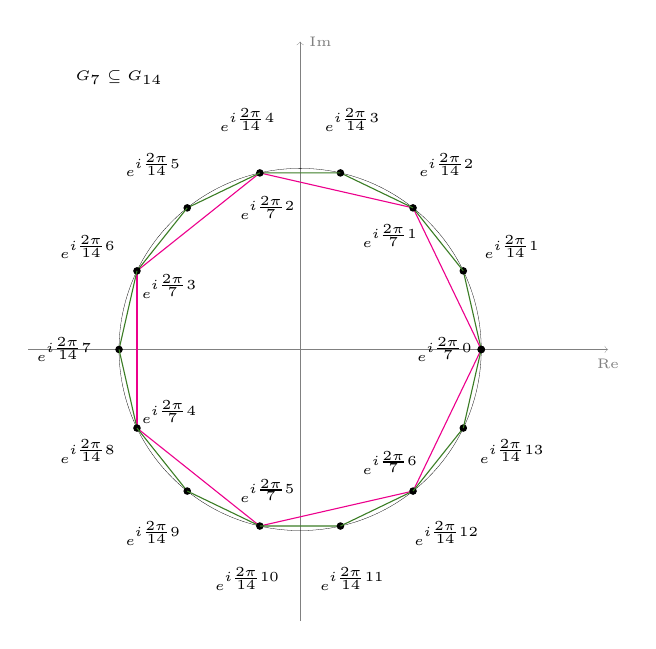
\begin{tikzpicture}[baseline=0,scale = 2.3, every node/.style={font=\tiny}]
  \draw[ultra thin,->,gray] (-1.5,0) -- (1.7,0) node[below] {Re};
  \draw[ultra thin,->,gray] (0,-1.5) -- (0,1.7) node[right] {Im};
  \draw[ultra thin] (0,0) circle (1);
  \node at (-1,1.5)  {$G_7 \subseteq G_{14}$};
  \foreach \x in {0,...,14} {
      \filldraw (\x*360/14:1) circle (0.5pt);
      \ifnum\x<14
        \draw[OliveGreen] (\x*360/14:1) -- ({(\x+1)*360/14}:1);
        \ifnum\x>0
          \filldraw (\x*360/14:1.3) node { $e^{i\frac{2\pi}{14}\x}$};
        \fi
      \fi
      \ifnum\x<7
        \filldraw (\x*360/7:0.8) node { $e^{i\frac{2\pi}{7}\x}$};
        \draw[magenta] (\x*360/7:1) -- ({(\x+1)*360/7}:1);
      \fi
    }
\end{tikzpicture}
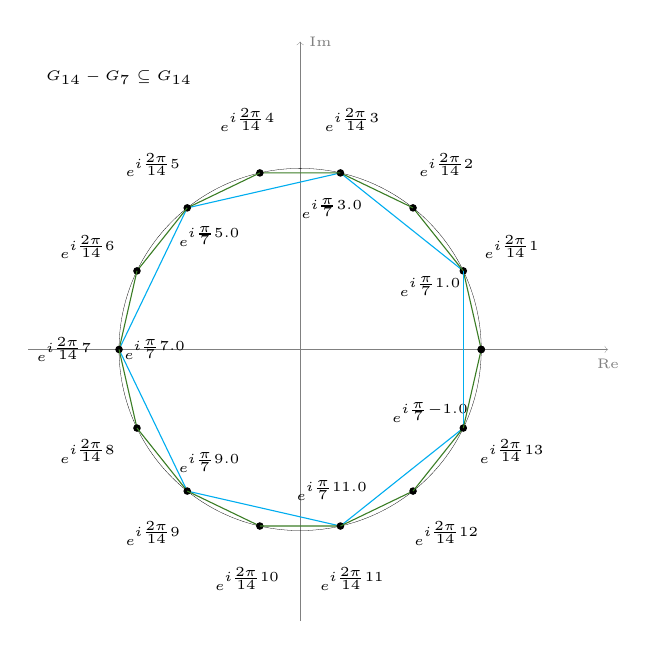
\begin{tikzpicture}[baseline=0,scale = 2.3, every node/.style={font=\tiny}]
  \draw[ultra thin,->,gray] (-1.5,0) -- (1.7,0) node[below] {Re};
  \draw[ultra thin,->,gray] (0,-1.5) -- (0,1.7) node[right] {Im};
  \draw[ultra thin] (0,0) circle (1);
  \node at (-1,1.5)  {$G_{14} - G_7 \subseteq G_{14}$};
  \foreach \x in {0,...,14} {
      \filldraw (\x*360/14:1) circle (0.5pt);
      \ifnum\x<14
        \draw[OliveGreen] (\x*360/14:1) -- ({(\x+1)*360/14}:1);
        \ifnum\x>0
          \filldraw (\x*360/14:1.3) node { $e^{i\frac{2\pi}{14}\x}$};
        \fi
      \fi
      \ifnum\x<7
        \draw[cyan] ({\x*360/7+360/14}:1) -- ({(\x+1)*360/7+360/14}:1);
        % \ifnum\x>0
        \filldraw ({\x*360/7 - 360/14}:0.8) node { $e^{i\frac{\pi}{7}\pgfmathparse{2*\x-1}\pgfmathresult}$ };
        % \fi
      \fi
    }
\end{tikzpicture}\\
